%%%%%%%%%%%%%%%%%%%%%%%%%%%%%%%%%%%%%%%%%


\documentclass[paper=a4, fontsize=11pt]{article} % A4 paper and 11pt font size

\usepackage{amsmath,amsfonts,amsthm} % Math packages
\usepackage{graphicx}


%\usepackage{fancyhdr} % Custom headers and footers
\pagestyle{plain} % Makes all pages in the document conform to the custom headers and footers

\title{	
Machine Learning \\
Homework 1
}

\author{Yao Song\\301266041} % Your name

\date{\normalsize\today} % Today's date or a custom date

\begin{document}

\maketitle % Print the title

%----------------------------------------------------------------------------------------
%	PROBLEM 1
%----------------------------------------------------------------------------------------

\section{Question 1}
\subsection{ML estimate of $\mu$}

\begin{align}
&\operatorname*{arg\,max}_{\mu} P({x_1,x_2,...,x_N}|\mu) \\
&= \operatorname*{arg\,max}_{\mu} P(x_1|\mu) P(x_2|\mu)... P(x_N|\mu)\\
&=\operatorname*{arg\,max}_{\mu} \exp \left\lbrace -\frac{1}{2\sigma^2} [(x_1 -\mu)^2+(x_2 -\mu)^2 +...+(x_N -\mu)^2]\right\rbrace\\
&=\operatorname*{arg\,min}_{\mu} [(x_1 -\mu)^2+(x_2 -\mu)^2 +...+(x_N -\mu)^2].
\end{align}
Define $f(\mu)  = (x_1 -\mu)^2+(x_2 -\mu)^2 +...+(x_N -\mu)^2$.\\
Let $\nabla_{\mu} f(\mu)  = -2(\sum_i x_i - N\mu) = 0$, we get 
$\mu_{ML} = \frac{1}{N}\sum_{i=1}^N x_i$.
\subsection{MAP estimate of $\mu$}
\begin{align}
&\operatorname*{arg\,max}_{\mu} P(\mu|D) 
=\operatorname*{arg\,max}_{\mu} P(\mu)P(D|\mu) \\
&=\operatorname*{arg\,max}_{\mu} \exp \left\lbrace -\frac{1}{2\sigma^2} [(x_1 -\mu)^2+(x_2 -\mu)^2 +...+(x_N -\mu)^2 + (a-\mu)^2]\right\rbrace\\
&=\operatorname*{arg\,min}_{\mu} [(x_1 -\mu)^2+(x_2 -\mu)^2 +...+(x_N -\mu)^2 +(a-\mu)^2]].
\end{align}
Like the ML estimate case, by taking derivative of the polynomial of $\mu$, we get 
$\mu_{MAP} = \frac{1}{N+1}(a + \sum_{i=1}^N x_i ) $
\subsection{what the prior mean a does in the MAP case}
The MAP estimate is a linear interpolation of the prior mean and the sample mean. 
The prior mean a help to adjust the sample mean estimate.

\subsection{effect of a much smaller $\sigma^2_p$}
If the prior distribution has a much smaller variance, than the MAP estimate will be much closer to the prior mean value a. Basically that means we have a quite confident prior distribution, much more confident than the likelihood distribution.


\section{Question 2}
\subsection{optimal weights $\boldsymbol{\omega}$}


Take gradient of the weighted sum of squares error function, we get the following equation:
\begin{align}
\boldsymbol{\nabla}_{\boldsymbol{\omega}} E(\boldsymbol{\omega})  = -\sum_{n=1}^N \alpha_n (t_n -\boldsymbol{\omega}^T \boldsymbol{\phi}(x_n) ) \boldsymbol{\phi}(x_n)^T.
\end{align}
Set the gradient to be zero, we obtain the following equation:
\begin{align}\label{eq:aa}
\sum_{n=1}^N \alpha_n t_n \boldsymbol{\phi}(x_n)^T 
= 
\boldsymbol{\omega}^T \sum_{n=1}^N \alpha_n  \boldsymbol{\phi}(x_n)  \boldsymbol{\phi}(x_n)^T.
\end{align}
Thus
\begin{align}
\boldsymbol{\omega}^T
= (\sum_{n=1}^N \alpha_n t_n \boldsymbol{\phi}(x_n)^T )
(\sum_{n=1}^N \alpha_n  \boldsymbol{\phi}(x_n)  \boldsymbol{\phi}(x_n)^T)^{-1},
\end{align}
Define diagonal matrix $\textbf{A} = diag(\alpha_1, \alpha_2,...,\alpha_N)$, 
$\textbf{t}^T =[t_1,t_2,...,t_N]$,\\
$\boldsymbol{\Phi} = 
 \begin{pmatrix}
  \phi_1(x_1) & \phi_2(x_1) & \cdots & \phi_M(x_1) \\
  \phi_1(x_2) & \phi_2(x_2) & \cdots & \phi_M(x_2)\\
  \vdots  & \vdots  & \ddots & \vdots  \\
  \phi_1(x_N) & \phi_2(x_N) & \cdots & \phi_M(x_N)
 \end{pmatrix}$, then the Equation (\ref{eq:aa}) can be written as:
\begin{align}
\boldsymbol{\Phi}^T \textbf{A}  \boldsymbol{t} 
= \boldsymbol{\omega}^T 
\boldsymbol {\Phi}^T \textbf{A} \boldsymbol{\Phi},
\end{align}
Thus,
\begin{align}
\boldsymbol{\omega} =
(\boldsymbol {\Phi}^T \textbf{A} \boldsymbol{\Phi})^{-1}
\boldsymbol{\Phi}^T \textbf{A}  \boldsymbol{t} ,
\end{align}


\subsection{interpretation of weights $\alpha_n$}
In the Gaussian noise model, $\textbf{t} = \textbf{y(x,w)} + \boldsymbol{\epsilon}$,
$\alpha_n$ is the variance of the noise term $\epsilon_n$.
Thus, the likelihood function of the data is written as follows:
\begin{equation}
p( \boldsymbol{t} |\boldsymbol{w}, \boldsymbol{\alpha}) 
=
\prod_{n=1}^N \mathcal{N} (t_n|\boldsymbol{w}^T \boldsymbol{\phi(x_n)}, \alpha_n) 
\end{equation}
By taking $\log$ function over the above equation, the weighted sum of squares error function will arise.
$\alpha_n$ is the variance of the noise term.


\section{Question 3}
For any matrix A, by the definition of eigenvalue, $\lambda$ and eigenvector,$v$, we have the following equation:
\begin{equation}
A v = \lambda v,
\end{equation}
which is equivalent to 
\begin{equation}
A v - \lambda v = (A - \lambda I)v = 0,
\end{equation}
where I is the identity matrix with the same size as matrix A. 
By the fundamental theorem of linear algebra, if the above linear equation has a nonzero solution $v$, then $\det(A- \lambda I)  =0$.
\begin{equation}
\det(A- \lambda I)  = (\lambda_1 - \lambda)(\lambda_2 - \lambda)...(\lambda_n - \lambda)
\end{equation}
If we set $\lambda =0$, we get $\det A = \lambda_1 \lambda_2...\lambda_n$.




\section{Question 4}
\subsection{polynomial regression from degree 1 to 7}
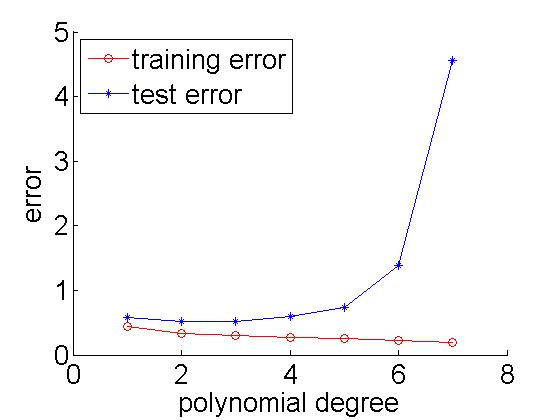
\includegraphics[width=\linewidth]{poly_reg.jpg}
Comment: 
The training error goes to zero as the polynomial degree increases.
The test error goes to the minimum and then increases as the polynomial degree increases.
This is due to over fitting in higher degrees.

\subsection{polynomial regression degree 1 weights}
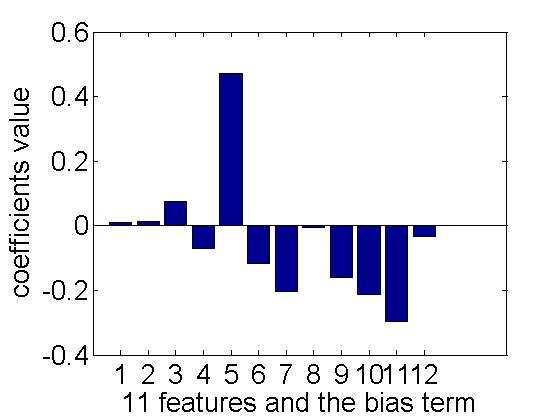
\includegraphics[width=\linewidth]{weights.jpg}
Comment:
The 5th feature has the largest positive value of the weight. A higher value of average number of rooms per dwelling implies a higher house value.
The 7th feature is negative. That means the feature has a negative effect on house value. That is reasonable because people prefer house near Boston employment center.
\subsection{1d vis}
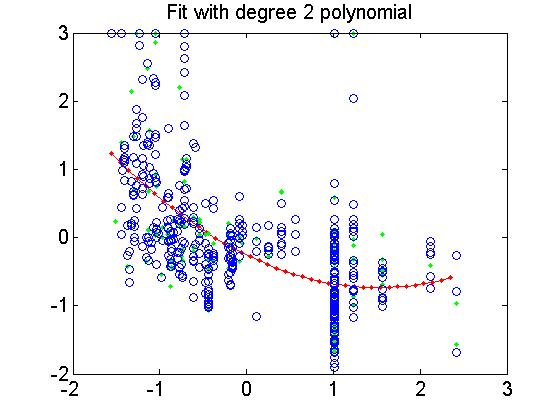
\includegraphics[width=\linewidth]{degree2_1d.jpg}
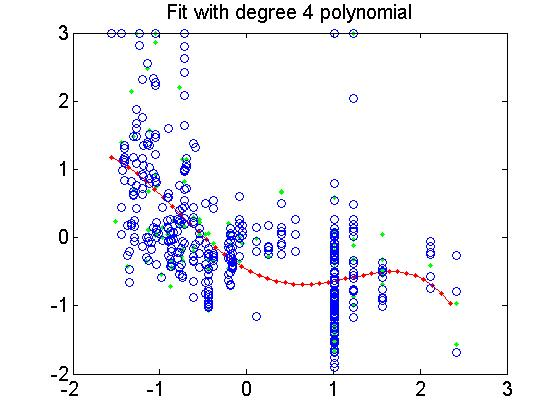
\includegraphics[width=\linewidth]{degree4_1d.jpg}
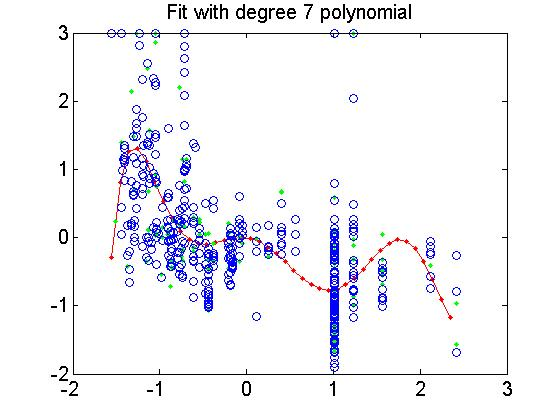
\includegraphics[width=\linewidth]{degree7_1d.jpg}
Comment: higher degree will give us a more complex curve. However, the points are so randomly distributed, the regression is still not well enough.

\subsection{polynomial regression regularized}
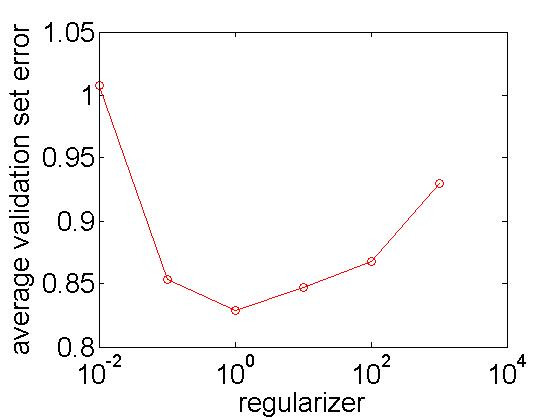
\includegraphics[width=\linewidth]{poly_reg_reg.jpg}
the case when $\lambda=0$ is not in the figure. When $\lambda  =0$, $error = 1.0550$. The best $\lambda$ is 1.


\subsection{Gaussian regression}
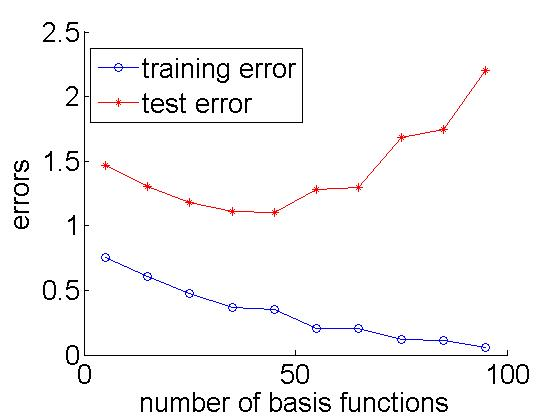
\includegraphics[width=\linewidth]{gaussian_regression.jpg}

comment: the training error goes down as the number of basis functions increase. The test error decreases to minimum then increases with number of basis functions. This is due to over fitting.

\subsection{Gaussian regression regularized}
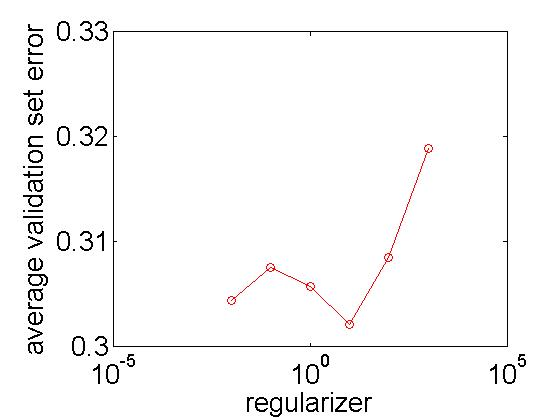
\includegraphics[width=\linewidth]{gaussian_reg_reg.jpg}

the case when $\lambda=0$ is not in the figure.when $\lambda=0$, $error = 0.3683$,which is much bigger than the ones in the figure.
The best $\lambda$ is 10.

\section{Question 5}
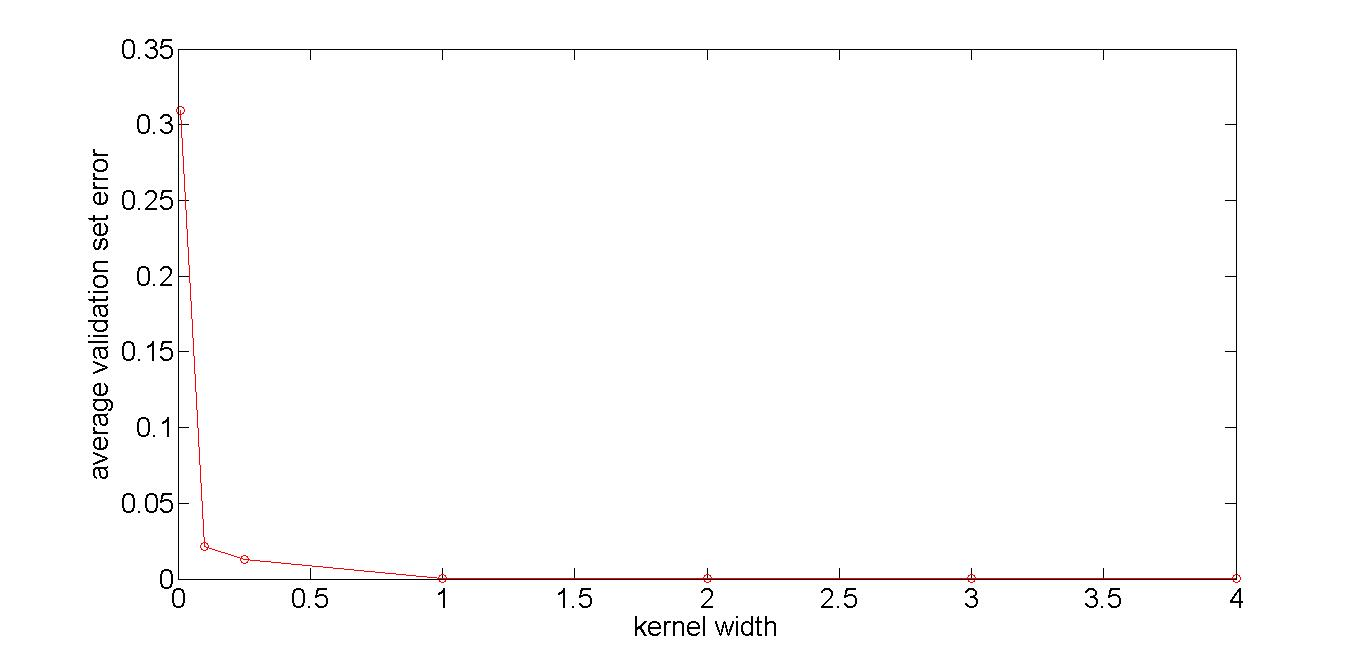
\includegraphics[width=\linewidth]{nadaray.jpg}
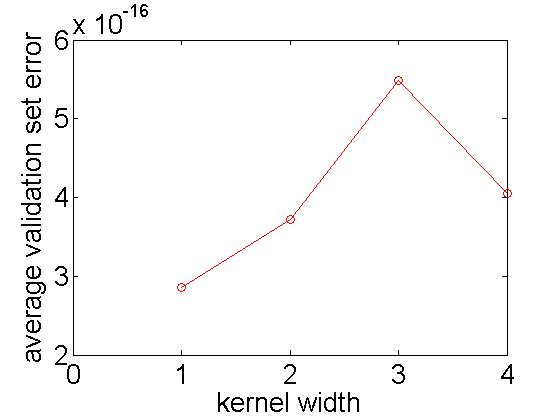
\includegraphics[width=\linewidth]{nadaray2.jpg}

The first figure shows all the values of h in the same figure. We can observe small values of h results in a higher estimation error.
This is because smaller h makes the kernel function to be zero. In that case, I just estimate the expected t value to be an average of the training t values.
The second figure zooms in to show the validation error when h =1,2,3,4. It is obvious that h = 1 is the best value.
%----------------------------------------------------------------------------------------

\end{document}